% !TEX root = ../main.tex
\section{Challenges}
\label{sec:problem}
In square fiducial marker detection, the pose is calculated by using the four corners of the tag. Since the tags are planar, it is easy to compute perspective point correspondences from the corners. This can be formalized as a specific case of the Perspective-N-Point problem and it has been well studied in geometry based Computer Vision literatures [][]. There are numerous optimization methods such as ones purposed in [] and [] to solve this problem. In particular, in [], the author shows that there is a deterministic solution to the Perspective-4-Point (P4P) problem. In other words, given the projection of a tag's 4 corners, the pose of the tag is unique. In practice, however, when a tag is captured in a low resolution camera, this method is very sensitive to noise. For instances, when ARTags, Apriltags and ARToolkit systems are used in scenarios shown in Figure \ref{fig:table_clearing}, the poses of the tags alter when the scene is static. Since the minimal number of perspective points are used to estimate the pose, a small variance in the corner detection process will yield estimations far from the true pose as shown in Figure \ref{fig:mismatch}.

We will illustrate the ambiguity effect by using two over lapping cubes in Figure \ref{fig:cube}. The overlapping face of the two cubes are interlaced but rotated by 120 degrees. However, due to perspective projection, the squares appears to be on the same plane. Under low camera resolution, the over lapping squares become virtually indistinguishable. The red circular regions are the detected corners under some sensory noise. Even though the reprojection error is minimized in the 2D space using P4P optimization methods, the 3D pose can still be far off. The result of the optimization can be characterized as a bimodal distribution and a function of the the viewing angle. Depending on the noise level in the scene, the optimization might converge to either one of the local minimum causing the pose estimation to be unreliable.
\begin{figure}
\centering
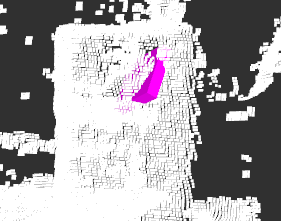
\includegraphics[width=\columnwidth]{figs/mismatch_tag}
\caption{The orientation of Apriltag placed on the object is greatly misaligned with the actual object}
\label{fig:mismatch}
\end{figure}

\begin{figure}
\centering
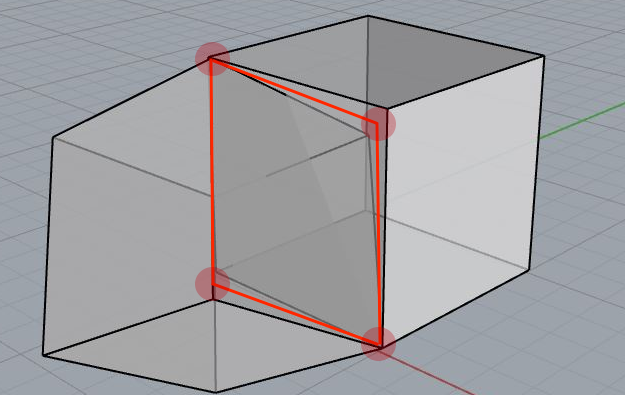
\includegraphics[width=\columnwidth]{figs/perspective_fig}
\caption{Perspective Ambiguity illustrated with overlapping cubes}
\label{fig:cube}
\end{figure}